\documentclass[12pt,a4paper]{article}
\usepackage[utf8]{inputenc}
\usepackage[T2A]{fontenc}
\usepackage[russian]{babel}
\usepackage{amsmath,amssymb,amsthm}
\usepackage{graphicx}
\usepackage{float}
\usepackage{listings}
\usepackage{xcolor}
\usepackage{geometry}
\usepackage{hyperref}
\usepackage{caption}

\geometry{left=2cm,right=2cm,top=2cm,bottom=2cm}

% Настройка листингов для Python
\lstset{
    language=Python,
    basicstyle=\ttfamily\small,
    keywordstyle=\color{blue}\bfseries,
    stringstyle=\color{red},
    commentstyle=\color{green! 60!black},
    morecomment=[l][\color{magenta}]{\#},
    numbers=left,
    numberstyle=\tiny\color{gray},
    stepnumber=1,
    numbersep=5pt,
    backgroundcolor=\color{gray!10},
    frame=single,
    rulecolor=\color{black},
    tabsize=4,
    breaklines=true,
    breakatwhitespace=true,
    showspaces=false,
    showstringspaces=false,
    captionpos=b,
    inputencoding=utf8,
    extendedchars=true,
    literate={а}{{\cyra}}1 {б}{{\cyrb}}1 {в}{{\cyrv}}1 {г}{{\cyrg}}1 {д}{{\cyrd}}1 
             {е}{{\cyre}}1 {ё}{{\cyryo}}1 {ж}{{\cyrzh}}1 {з}{{\cyrz}}1 {и}{{\cyri}}1 
             {й}{{\cyrishrt}}1 {к}{{\cyrk}}1 {л}{{\cyrl}}1 {м}{{\cyrm}}1 {н}{{\cyrn}}1 
             {о}{{\cyro}}1 {п}{{\cyrp}}1 {р}{{\cyrr}}1 {с}{{\cyrs}}1 {т}{{\cyrt}}1 
             {у}{{\cyru}}1 {ф}{{\cyrf}}1 {х}{{\cyrh}}1 {ц}{{\cyrc}}1 {ч}{{\cyrch}}1 
             {ш}{{\cyrsh}}1 {щ}{{\cyrshch}}1 {ъ}{{\cyrhrdsn}}1 {ы}{{\cyrery}}1 
             {ь}{{\cyrsftsn}}1 {э}{{\cyrerev}}1 {ю}{{\cyryu}}1 {я}{{\cyrya}}1
}

\title{\textbf{Расчётно-графическая работа №1 }}
\author{Ануфриев Андрей \\Вариант №3
}

\date{\today}

\begin{document}

\maketitle
\tableofcontents
\newpage

%=============================================================================
\section{Задание I.  Изобразить множество на комплексной плоскости}
%=============================================================================

\subsection{Условие}
Изобразить на комплексной плоскости множество $\mathcal{D}$:
\[
\mathcal{D} = \{z : 2 \leq |z + 2| < 3, \quad -\pi/2 < \arg z \leq \pi/2\}
\]

\subsection{Решение}

\textbf{Анализ условий:}

\textbf{Условие 1:} $2 \leq |z + 2| < 3$
\begin{itemize}
    \item $|z + 2|$ --- расстояние от точки $z$ до точки $-2$
    \item $|z + 2| \geq 2$ --- внешность круга радиуса 2 с центром в $(-2, 0)$, включая границу
    \item $|z + 2| < 3$ --- внутренность круга радиуса 3 с центром в $(-2, 0)$, не включая границу
    \item Вместе: \textbf{кольцо} с центром в $(-2, 0)$, внутренний радиус 2 (включён), внешний радиус 3 (не включён)
\end{itemize}

\textbf{Условие 2:} $-\pi/2 < \arg z \leq \pi/2$
\begin{itemize}
    \item $\arg z$ --- аргумент числа $z$ относительно начала координат
    \item Это \textbf{правая полуплоскость} $\text{Re}(z) \geq 0$
    \item Положительная мнимая полуось включена, отрицательная --- нет
\end{itemize}

\textbf{Границы:}
\begin{itemize}
    \item \textbf{Сплошная линия} ($\in \mathcal{D}$): дуга $|z+2| = 2$, луч $\arg z = \pi/2$
    \item \textbf{Пунктирная линия} ($\notin \mathcal{D}$): дуга $|z+2| = 3$, луч $\arg z = -\pi/2$
\end{itemize}

\subsection{График}
\begin{figure}[H]
    \centering
    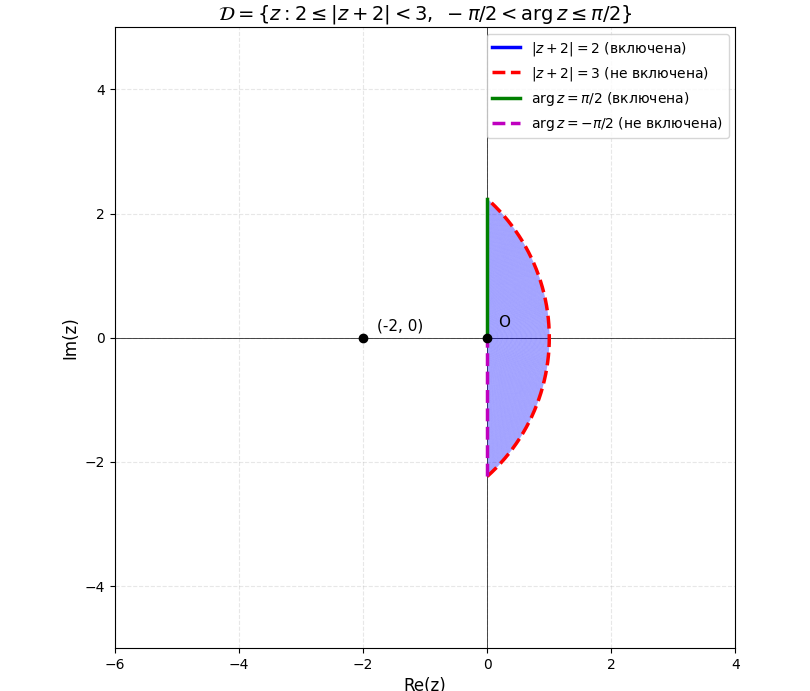
\includegraphics[width=0.7\textwidth]{Figure_1.png}
    \caption{Множество $\mathcal{D} = \{z : 2 \leq |z+2| < 3, -\pi/2 < \arg z \leq \pi/2\}$}
\end{figure}

\subsection{Листинг программы}
\begin{lstlisting}[caption={Построение множества D на комплексной плоскости}]
import numpy as np
import matplotlib. pyplot as plt

fig, ax = plt. subplots(figsize=(10, 10))
ax.set_aspect('equal')
ax.set_xlim(-6, 4)
ax.set_ylim(-5, 5)

center = (-2, 0)
r_inner, r_outer = 2, 3

# Заливка области
theta_range = np.linspace(-np.pi, np.pi, 1000)
for r in np.linspace(r_inner, r_outer, 200):
    x_ring = center[0] + r * np. cos(theta_range)
    y_ring = center[1] + r * np.sin(theta_range)
    mask = (x_ring >= 0) & ~((x_ring == 0) & (y_ring < 0))
    ax.plot(x_ring[mask], y_ring[mask], 'b-', linewidth=0.3, alpha=0.3)

# Внутренняя окружность (включена)
theta_full = np.linspace(0, 2*np.pi, 500)
x_inner = center[0] + r_inner * np.cos(theta_full)
y_inner = center[1] + r_inner * np.sin(theta_full)
mask_inner = x_inner >= 0
ax.plot(x_inner[mask_inner], y_inner[mask_inner], 'b-', linewidth=2)

# Внешняя окружность (не включена)
x_outer = center[0] + r_outer * np.cos(theta_full)
y_outer = center[1] + r_outer * np.sin(theta_full)
mask_outer = x_outer >= 0
ax.plot(x_outer[mask_outer], y_outer[mask_outer], 'r--', linewidth=2)

plt.savefig('complex_set_D.png', dpi=150)
plt.show()
\end{lstlisting}

\newpage
%=============================================================================
\section{Задание II. Найти все значения функции в указанной точке}
%=============================================================================

\subsection{Условие}
Найти все значения $\text{Ln}(1+i)$. 

\subsection{Решение}

\textbf{Определение комплексного логарифма:}
\[
\text{Ln}(z) = \ln|z| + i(\arg z + 2\pi k), \quad k \in \mathbb{Z}
\]

\textbf{Шаг 1. } Представим $z = 1 + i$ в показательной форме. 

Модуль:
\[
|z| = |1+i| = \sqrt{1^2 + 1^2} = \sqrt{2}
\]

Главное значение аргумента:
\[
\arg(1+i) = \arctan\left(\frac{1}{1}\right) = \frac{\pi}{4}
\]

\textbf{Шаг 2.} Вычисление логарифма:
\[
\text{Ln}(1+i) = \ln\sqrt{2} + i\left(\frac{\pi}{4} + 2\pi k\right), \quad k \in \mathbb{Z}
\]

\subsection{Ответ}
\[
\boxed{\text{Ln}(1+i) = \frac{1}{2}\ln 2 + i\left(\frac{\pi}{4} + 2\pi k\right), \quad k \in \mathbb{Z}}
\]

Главное значение ($k = 0$):
\[
\ln(1+i) = \frac{\ln 2}{2} + i\frac{\pi}{4} \approx 0. 3466 + 0. 7854i
\]

% \subsection{Листинг программы}
% \begin{lstlisting}[caption={Вычисление комплексного логарифма}]
% import numpy as np

% z = 1 + 1j
% modulus = np.abs(z)
% arg_principal = np.angle(z)

% print(f"z = {z}")
% print(f"|z| = {modulus:. 6f}")
% print(f"arg(z) = {arg_principal:.6f}")

% ln_modulus = np.log(modulus)
% print(f"ln|z| = {ln_modulus:.6f}")

% print(f"\nLn(1+i) = {ln_modulus:.4f} + i*(pi/4 + 2*pi*k)")

% for k in range(-2, 3):
%     value = ln_modulus + 1j * (arg_principal + 2 * np.pi * k)
%     print(f"k = {k:2d}: {value. real:.4f} + {value.imag:.4f}i")
% \end{lstlisting}

\newpage
%=============================================================================
\section{Задание III.  Найти аналитическую функцию по известной части}
%=============================================================================

\subsection{Условие}
Найти аналитическую функцию по известной мнимой части:
\[
v(x, y) = \exp\left(-\frac{y}{2}\right) \cos\frac{x}{2} - \frac{y^3}{3} + x^2 y
\]

\subsection{Решение}

\textbf{Условия Коши-Римана:}
\[
\frac{\partial u}{\partial x} = \frac{\partial v}{\partial y}, \quad \frac{\partial u}{\partial y} = -\frac{\partial v}{\partial x}
\]

\textbf{Шаг 1.} Вычислим частные производные $v(x,y)$:
\[
\frac{\partial v}{\partial x} = -\frac{1}{2}e^{-y/2}\sin\frac{x}{2} + 2xy
\]
\[
\frac{\partial v}{\partial y} = -\frac{1}{2}e^{-y/2}\cos\frac{x}{2} - y^2 + x^2
\]

\textbf{Шаг 2.} Из $\frac{\partial u}{\partial x} = \frac{\partial v}{\partial y}$ интегрируем по $x$:
\[
u = -e^{-y/2}\sin\frac{x}{2} + \frac{x^3}{3} - xy^2 + \varphi(y)
\]

\textbf{Шаг 3. } Из условия $\frac{\partial u}{\partial y} = -\frac{\partial v}{\partial x}$ находим $\varphi'(y) = 0$, то есть $\varphi(y) = C$. 

\textbf{Шаг 4.} Переход к комплексной переменной:
\begin{itemize}
    \item $ie^{iz/2} = -e^{-y/2}\sin\frac{x}{2} + ie^{-y/2}\cos\frac{x}{2}$
    \item $\frac{z^3}{3} = \frac{x^3}{3} - xy^2 + i\left(x^2y - \frac{y^3}{3}\right)$
\end{itemize}

\subsection{Ответ}
\[
\boxed{f(z) = \frac{z^3}{3} + ie^{iz/2} + C, \quad C \in \mathbb{R}}
\]

% \subsection{Листинг программы}
% \begin{lstlisting}[caption={Проверка аналитической функции}]
% import numpy as np

% def v_given(x, y):
%     return np.exp(-y/2) * np.cos(x/2) - y**3/3 + x**2 * y

% def u_found(x, y, C=0):
%     return -np.exp(-y/2) * np.sin(x/2) + x**3/3 - x * y**2 + C

% def f_complex(z, C=0):
%     return z**3 / 3 + 1j * np.exp(1j * z / 2) + C

% # Проверка условий Коши-Римана
% h = 1e-7
% x0, y0 = 1. 5, 0.8

% du_dx = (u_found(x0+h, y0) - u_found(x0-h, y0)) / (2*h)
% dv_dy = (v_given(x0, y0+h) - v_given(x0, y0-h)) / (2*h)
% print(f"du/dx = {du_dx:. 6f}, dv/dy = {dv_dy:.6f}")
% \end{lstlisting}

\newpage
%=============================================================================
\section{Задание IV.  Вычислить интеграл по заданной кривой}
%=============================================================================

\subsection{Условие}
\[
\int_C x \, dz
\]
где $C$ --- полуокружность $|z| = 1$, $0 \leq \arg z \leq \pi$.  Начало пути в точке $z = 1$.

\subsection{Решение}

\textbf{Шаг 1.} Параметризация контура:
\[
z(t) = e^{it} = \cos t + i\sin t, \quad t \in [0, \pi]
\]
\[
x = \cos t, \quad dz = ie^{it} \, dt
\]

\textbf{Шаг 2.} Подстановка в интеграл:
\[
\int_C x \, dz = \int_0^{\pi} \cos t \cdot ie^{it} \, dt = i \int_0^{\pi} \cos t \cdot e^{it} \, dt
\]

\textbf{Шаг 3. } Вычисление:
\[
\int_0^{\pi} \cos t \cdot e^{it} \, dt = \int_0^{\pi} \cos^2 t \, dt + i \int_0^{\pi} \cos t \sin t \, dt = \frac{\pi}{2} + 0 = \frac{\pi}{2}
\]

\textbf{Шаг 4.} Результат:
\[
\int_C x \, dz = i \cdot \frac{\pi}{2} = \frac{\pi i}{2}
\]

\subsection{Ответ}
\[
\boxed{\int_C x \, dz = \frac{\pi i}{2}}
\]

\subsection{График}
\begin{figure}[H]
    \centering
    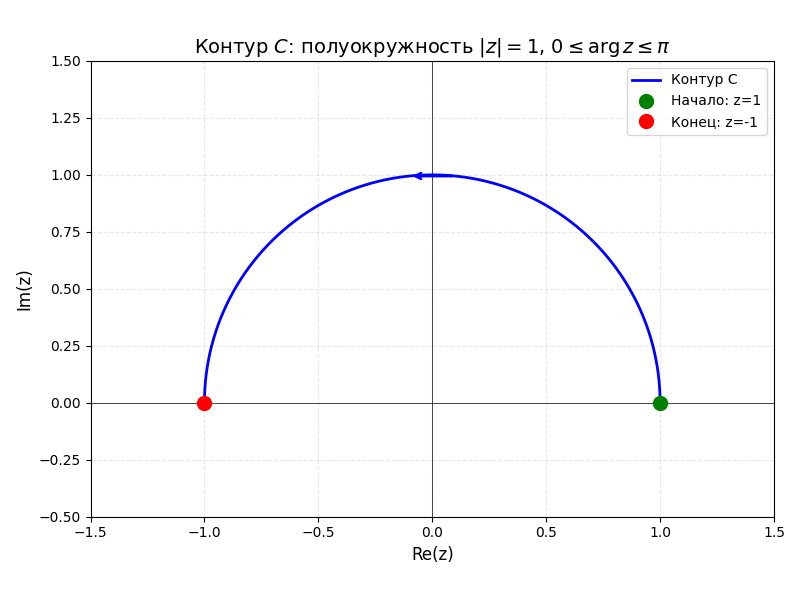
\includegraphics[width=0.6\textwidth]{Figure_4.png}
    \caption{Контур интегрирования: верхняя полуокружность $|z|=1$}
\end{figure}

\subsection{Листинг программы}
\begin{lstlisting}[caption={Вычисление криволинейного интеграла}]
import numpy as np
from scipy import integrate

def integrand_real(t):
    return np.cos(t) * np.cos(t)

def integrand_imag(t):
    return np.cos(t) * np.sin(t)

real_part, _ = integrate.quad(integrand_real, 0, np. pi)
imag_part, _ = integrate.quad(integrand_imag, 0, np. pi)

result = 1j * (real_part + 1j * imag_part)
print(f"Integral = {result.real:.6f} + {result.imag:.6f}i")
print(f"pi/2 = {np.pi/2:.6f}")
\end{lstlisting}

\newpage
%=============================================================================
\section{Задание V.  Разложить функцию в ряд Тейлора}
%=============================================================================

\subsection{Условие}
Разложить функцию $f(z) = (z+1)(z-2)^{-1}$ в ряд Тейлора в окрестности точки $z_0 = 1$ и указать область сходимости. 

\subsection{Решение}

\textbf{Шаг 1.} Преобразование функции:
\[
f(z) = \frac{z+1}{z-2}
\]

Замена $w = z - 1$:
\[
f(z) = \frac{w+2}{w-1} = 1 + \frac{3}{w-1}
\]

\textbf{Шаг 2.} Разложение:
\[
\frac{1}{w-1} = -\frac{1}{1-w} = -\sum_{n=0}^{\infty} w^n, \quad |w| < 1
\]

\textbf{Шаг 3.} Подставляем:
\[
f(z) = 1 - 3\sum_{n=0}^{\infty} (z-1)^n = -2 - 3(z-1) - 3(z-1)^2 - 3(z-1)^3 - \ldots
\]

\textbf{Область сходимости:} ближайшая особая точка --- полюс $z = 2$, расстояние $|2 - 1| = 1$. 

\subsection{Ответ}
\[
\boxed{f(z) = -2 - 3\sum_{n=1}^{\infty}(z-1)^n}
\]
\[
\boxed{\text{Область сходимости: } |z-1| < 1}
\]

\subsection{График}
\begin{figure}[H]
    \centering
    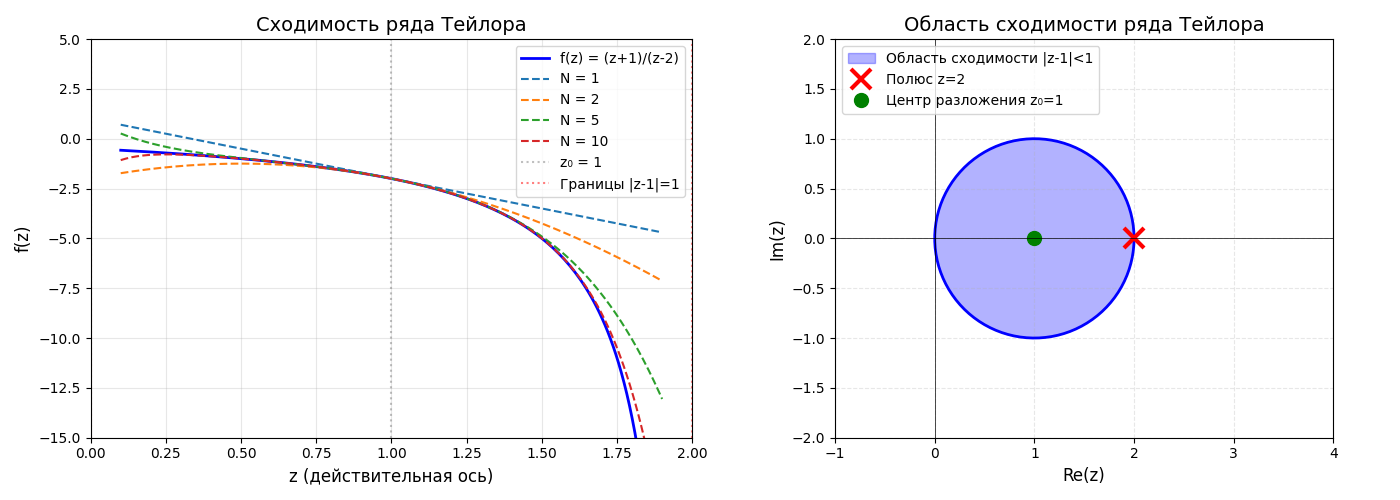
\includegraphics[width=\textwidth]{Figure_2.png}
    \caption{Сходимость ряда Тейлора и область сходимости}
\end{figure}

\subsection{Листинг программы}
\begin{lstlisting}[caption={Разложение в ряд Тейлора}]
import numpy as np

def f(z):
    return (z + 1) / (z - 2)

def taylor_sum(z, z0, N):
    w = z - z0
    return -2 - 3 * sum(w**n for n in range(1, N+1))

z0 = 1
test_points = [0. 5, 0.8, 1.0, 1.2, 1.5]

for z in test_points:
    exact = f(z)
    approx = taylor_sum(z, z0, 20)
    print(f"z={z}: f(z)={exact:.6f}, Taylor={approx:.6f}")
\end{lstlisting}

\newpage
%=============================================================================
\section{Задание VI. Разложить функцию в ряд Лорана}
%=============================================================================

\subsection{Условие}
Разложить функцию в ряд Лорана в указанной области:
\[
f(z) = \left(\frac{3z}{2} - \frac{1}{z}\right) \cos\frac{1}{z}, \quad 0 < |z| < \infty
\]

\subsection{Решение}

\textbf{Шаг 1.} Разложение $\cos\frac{1}{z}$:
\[
\cos\frac{1}{z} = \sum_{n=0}^{\infty} \frac{(-1)^n}{(2n)!} \cdot \frac{1}{z^{2n}} = 1 - \frac{1}{2!  z^2} + \frac{1}{4! z^4} - \ldots
\]

\textbf{Шаг 2.} Умножаем на $\frac{3z}{2}$:
\[
\frac{3z}{2} \cos\frac{1}{z} = \frac{3z}{2} - \frac{3}{4z} + \frac{1}{16z^3} - \ldots
\]

\textbf{Шаг 3.} Умножаем на $-\frac{1}{z}$:
\[
-\frac{1}{z} \cos\frac{1}{z} = -\frac{1}{z} + \frac{1}{2z^3} - \frac{1}{24z^5} + \ldots
\]

\textbf{Шаг 4.} Складываем и получаем коэффициенты:
\begin{itemize}
    \item $c_1 = \frac{3}{2}$
    \item $c_{-1} = -\frac{3}{4} - 1 = -\frac{7}{4}$
    \item $c_{-3} = \frac{1}{16} + \frac{1}{2} = \frac{9}{16}$
    \item $c_{-5} = -\frac{7}{160}$
\end{itemize}

\textbf{Особая точка:} $z = 0$ --- существенно особая (главная часть содержит бесконечно много членов).

\subsection{Ответ}
\[
\boxed{f(z) = \frac{3}{2}z - \frac{7}{4z} + \frac{9}{16z^3} - \frac{7}{160z^5} + \ldots}
\]

\subsection{График}
\begin{figure}[H]
    \centering
    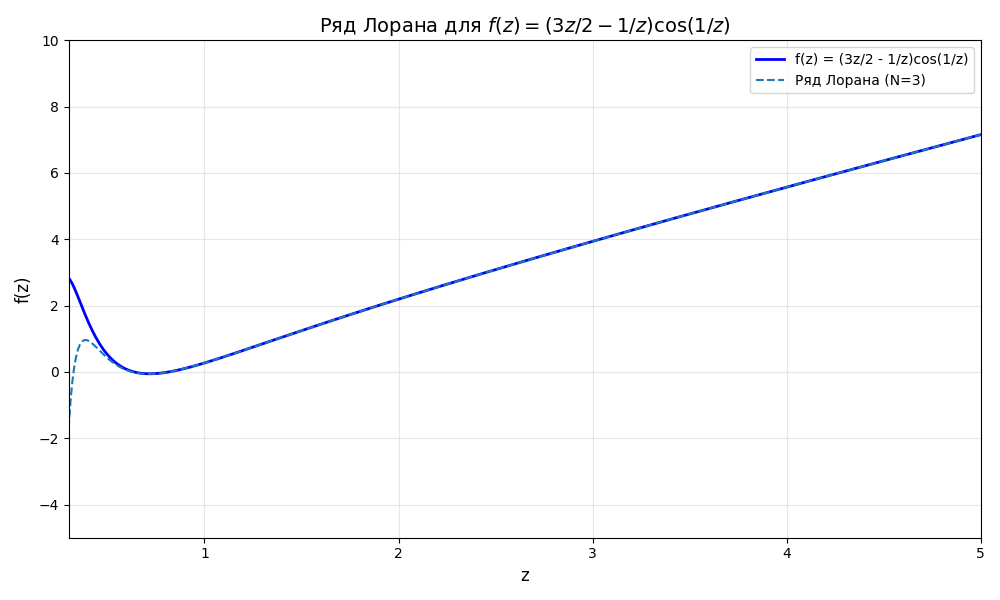
\includegraphics[width=0.7\textwidth]{Figure_6.png}
    \caption{Ряд Лорана для $f(z) = (3z/2 - 1/z)\cos(1/z)$}
\end{figure}

\subsection{Листинг программы}
\begin{lstlisting}[caption={Разложение в ряд Лорана}]
import numpy as np
from math import factorial

def f(z):
    return (3*z/2 - 1/z) * np.cos(1/z)

def laurent_sum(z, N_terms=15):
    result = 0
    for n in range(N_terms):
        result += (3/2) * ((-1)**n) / factorial(2*n) * z**(1-2*n)
        result += -((-1)**n) / factorial(2*n) * z**(-1-2*n)
    return result

test_points = [0.5, 1.0, 2.0, 3.0, 5.0]
for z in test_points:
    exact = f(z)
    approx = laurent_sum(z, 15)
    print(f"z={z}: f(z)={exact:.6f}, Laurent={approx:.6f}")
\end{lstlisting}

\newpage
%=============================================================================
\section{Задание VII. Вычислить интеграл при помощи вычетов}
%=============================================================================

\subsection{Условие}
\[
\oint_L \frac{dz}{z^4 + 2z^3}, \quad L = \{z : |z| = 3\}
\]

\subsection{Решение}

\textbf{Шаг 1.} Упрощение:
\[
f(z) = \frac{1}{z^4 + 2z^3} = \frac{1}{z^3(z + 2)}
\]

\textbf{Шаг 2.} Особые точки внутри контура $|z| = 3$:
\begin{itemize}
    \item $z = 0$ --- полюс 3-го порядка, $|0| = 0 < 3$ \checkmark
    \item $z = -2$ --- простой полюс, $|-2| = 2 < 3$ \checkmark
\end{itemize}

\textbf{Шаг 3.} Вычет в $z = -2$ (полюс 1-го порядка):
\[
\text{Res}_{z=-2} f(z) = \lim_{z \to -2} (z+2) \cdot \frac{1}{z^3(z+2)} = \frac{1}{(-2)^3} = -\frac{1}{8}
\]

\textbf{Шаг 4.} Вычет в $z = 0$ (полюс 3-го порядка):
\[
\text{Res}_{z=0} f(z) = \frac{1}{2! } \lim_{z \to 0} \frac{d^2}{dz^2}\left[\frac{1}{z+2}\right] = \frac{1}{2} \cdot \frac{2}{8} = \frac{1}{8}
\]

\textbf{Шаг 5. } Сумма вычетов:
\[
\sum \text{Res} = \frac{1}{8} + \left(-\frac{1}{8}\right) = 0
\]

\subsection{Ответ}
\[
\boxed{\oint_L \frac{dz}{z^4 + 2z^3} = 2\pi i \cdot 0 = 0}
\]

\subsection{График}
\begin{figure}[H]
    \centering
    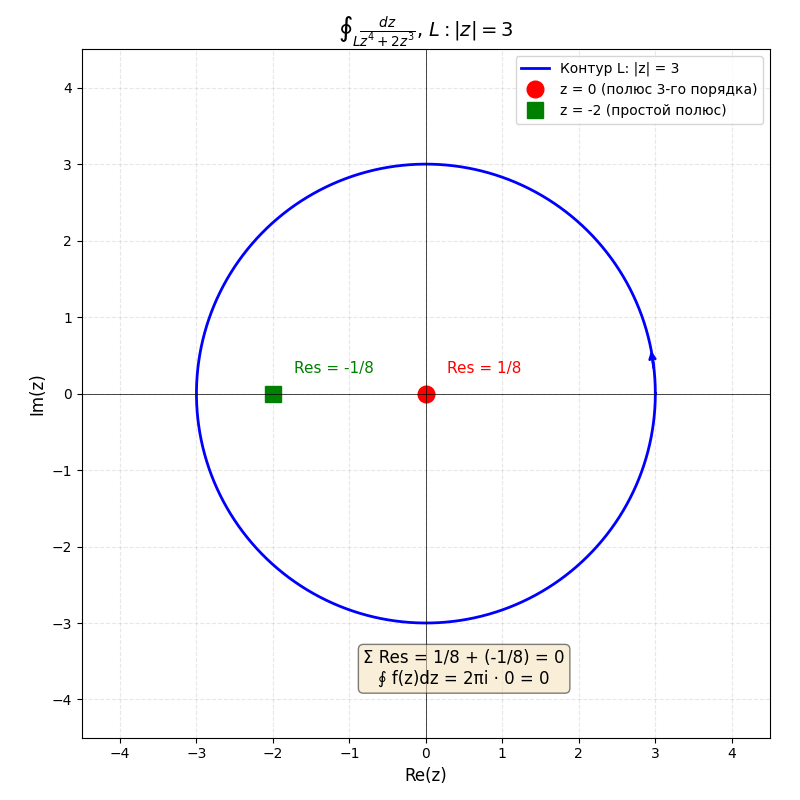
\includegraphics[width=0.6\textwidth]{Figure_7.png}
    \caption{Контур интегрирования и особые точки}
\end{figure}

\subsection{Листинг программы}
\begin{lstlisting}[caption={Вычисление интеграла методом вычетов}]
import numpy as np
from scipy import integrate

def f(z):
    return 1 / (z**4 + 2*z**3)

# Вычеты
res_minus2 = 1 / ((-2)**3)  # = -1/8
res_0 = 1/8

print(f"Res[f, z=-2] = {res_minus2}")
print(f"Res[f, z=0] = {res_0}")
print(f"Sum = {res_0 + res_minus2}")
print(f"Integral = 2*pi*i * {res_0 + res_minus2} = 0")
\end{lstlisting}

\newpage
%=============================================================================
\section{Задание VIII. Вычислить несобственный интеграл}
%=============================================================================

\subsection{Условие}
\[
\int_{-\infty}^{+\infty} \frac{x \sin(ax)}{x^2 + 2x + 10} \, dx, \quad a > 0
\]

\subsection{Решение}

\textbf{Шаг 1.} Используем формулу:
\[
\int_{-\infty}^{+\infty} f(x) \sin(ax) \, dx = \text{Im} \int_{-\infty}^{+\infty} f(x) e^{iax} \, dx
\]

Рассмотрим:
\[
I = \int_{-\infty}^{+\infty} \frac{x \, e^{iax}}{x^2 + 2x + 10} \, dx
\]

\textbf{Шаг 2.} Полюсы знаменателя $x^2 + 2x + 10 = 0$:
\[
z_{1,2} = \frac{-2 \pm \sqrt{4-40}}{2} = -1 \pm 3i
\]

В верхней полуплоскости: $z_1 = -1 + 3i$. 

\textbf{Шаг 3.} Вычет в $z_1 = -1 + 3i$:
\[
\text{Res}_{z=z_1} f(z) = \frac{z_1 \, e^{iaz_1}}{z_1 - z_2} = \frac{(-1+3i) \cdot e^{-3a-ia}}{6i}
\]

\textbf{Шаг 4.} После вычислений:
\[
I = 2\pi i \cdot \text{Res}_{z=z_1} = \frac{\pi e^{-3a}}{3}\left[(3\sin a - \cos a) + i(\sin a + 3\cos a)\right]
\]

\textbf{Шаг 5.} Мнимая часть:
\[
\int_{-\infty}^{+\infty} \frac{x \sin(ax)}{x^2 + 2x + 10} \, dx = \text{Im}(I) = \frac{\pi e^{-3a}}{3}(\sin a + 3\cos a)
\]

\subsection{Ответ}
\[
\boxed{\int_{-\infty}^{+\infty} \frac{x \sin(ax)}{x^2 + 2x + 10} \, dx = \frac{\pi e^{-3a}}{3}(\sin a + 3\cos a), \quad a > 0}
\]

\subsection{График}
\begin{figure}[H]
    \centering
    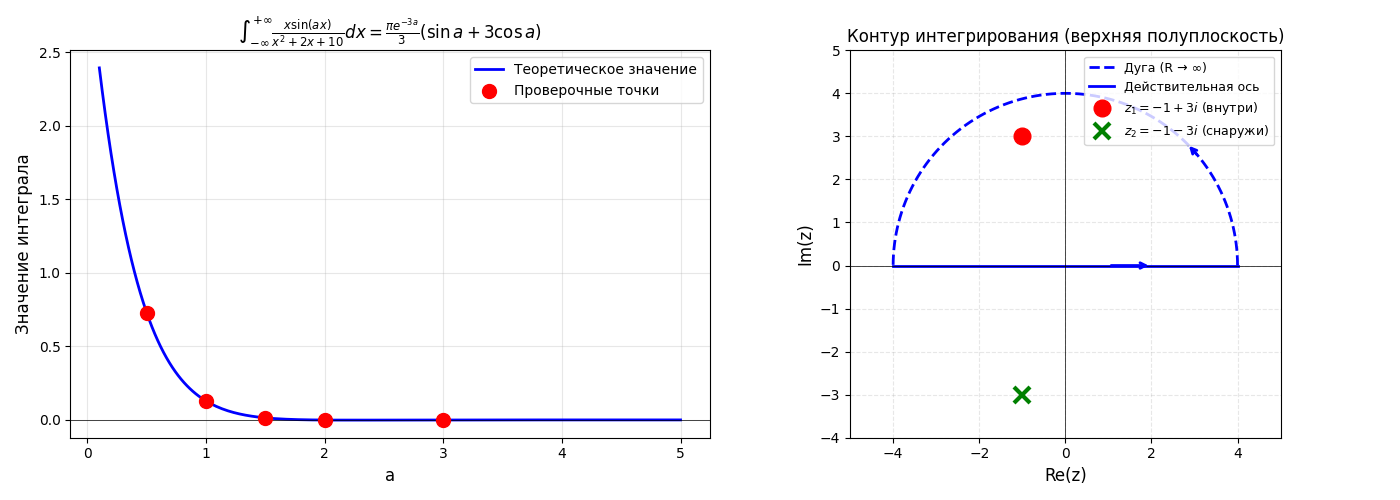
\includegraphics[width=\textwidth]{Figure_8.png}
    \caption{Зависимость интеграла от параметра $a$ и контур интегрирования}
\end{figure}

\subsection{Листинг программы}
\begin{lstlisting}[caption={Вычисление несобственного интеграла}]
import numpy as np
from scipy import integrate

def theoretical_result(a):
    return (np.pi / 3) * np.exp(-3*a) * (np.sin(a) + 3*np.cos(a))

def integrand(x, a):
    return x * np.sin(a * x) / (x**2 + 2*x + 10)

a_values = [0.5, 1.0, 1.5, 2.0]
for a in a_values:
    theor = theoretical_result(a)
    print(f"a = {a}: I = {theor:. 6f}")
\end{lstlisting}

\end{document}